\documentclass[12pt,a4paper]{article}
\usepackage[margin=1in]{geometry}
\usepackage[moduleName=2612]{KautenjaDSP}
% import a debugging package to show the margin boxes
% \usepackage{showframe}
% set the graphics path to the img directory
\graphicspath{{img/}}

% algorithm2e stuff
% \SetKwInOut{Objects}{$\CKmatrix{O}$}
% \SetKwInOut{Weights}{$\CKvector{w}$}

\begin{document}
\titlePage{2612-Logo}{2612-Module}{KautenjaDSP}

% -------------------
% MARK: Overview
% -------------------

\section{Overview}

2612 is an emulation of the Yamaha YM2612 audio processing unit from the Sega Master System and Sega Genesis for VCV Rack. The YM2612 is a 4-operator FM synthesis chip with 6 voices of polyphony.

2612 provides the key features of the 2612 chip, namely,
\begin{itemize}
  \item \textbf{16-bit:} 8 bits better than the previous generation of chips!
  \item \textbf{6 Voice Polyphony:} 6 voices of polyphony with independent V/OCT and Gate inputs
  \item \textbf{4-Operator FM Synthesis:} Full control over the FM-synthesis parameters for each of the four operators including: envelopes, multiplier rate scale, tuning, and amplitude modulation
  \item \textbf{8 FM Algorithms:} 8 different arrangements of the four operators
  \item \textbf{Stereo Outputs:} Output from the left and right channels on the chip
\end{itemize}

% -------------------
% MARK: Panel Layout
% -------------------

\clearpage
\section{Panel Layout}

\begin{figure}[!htp]
\centering
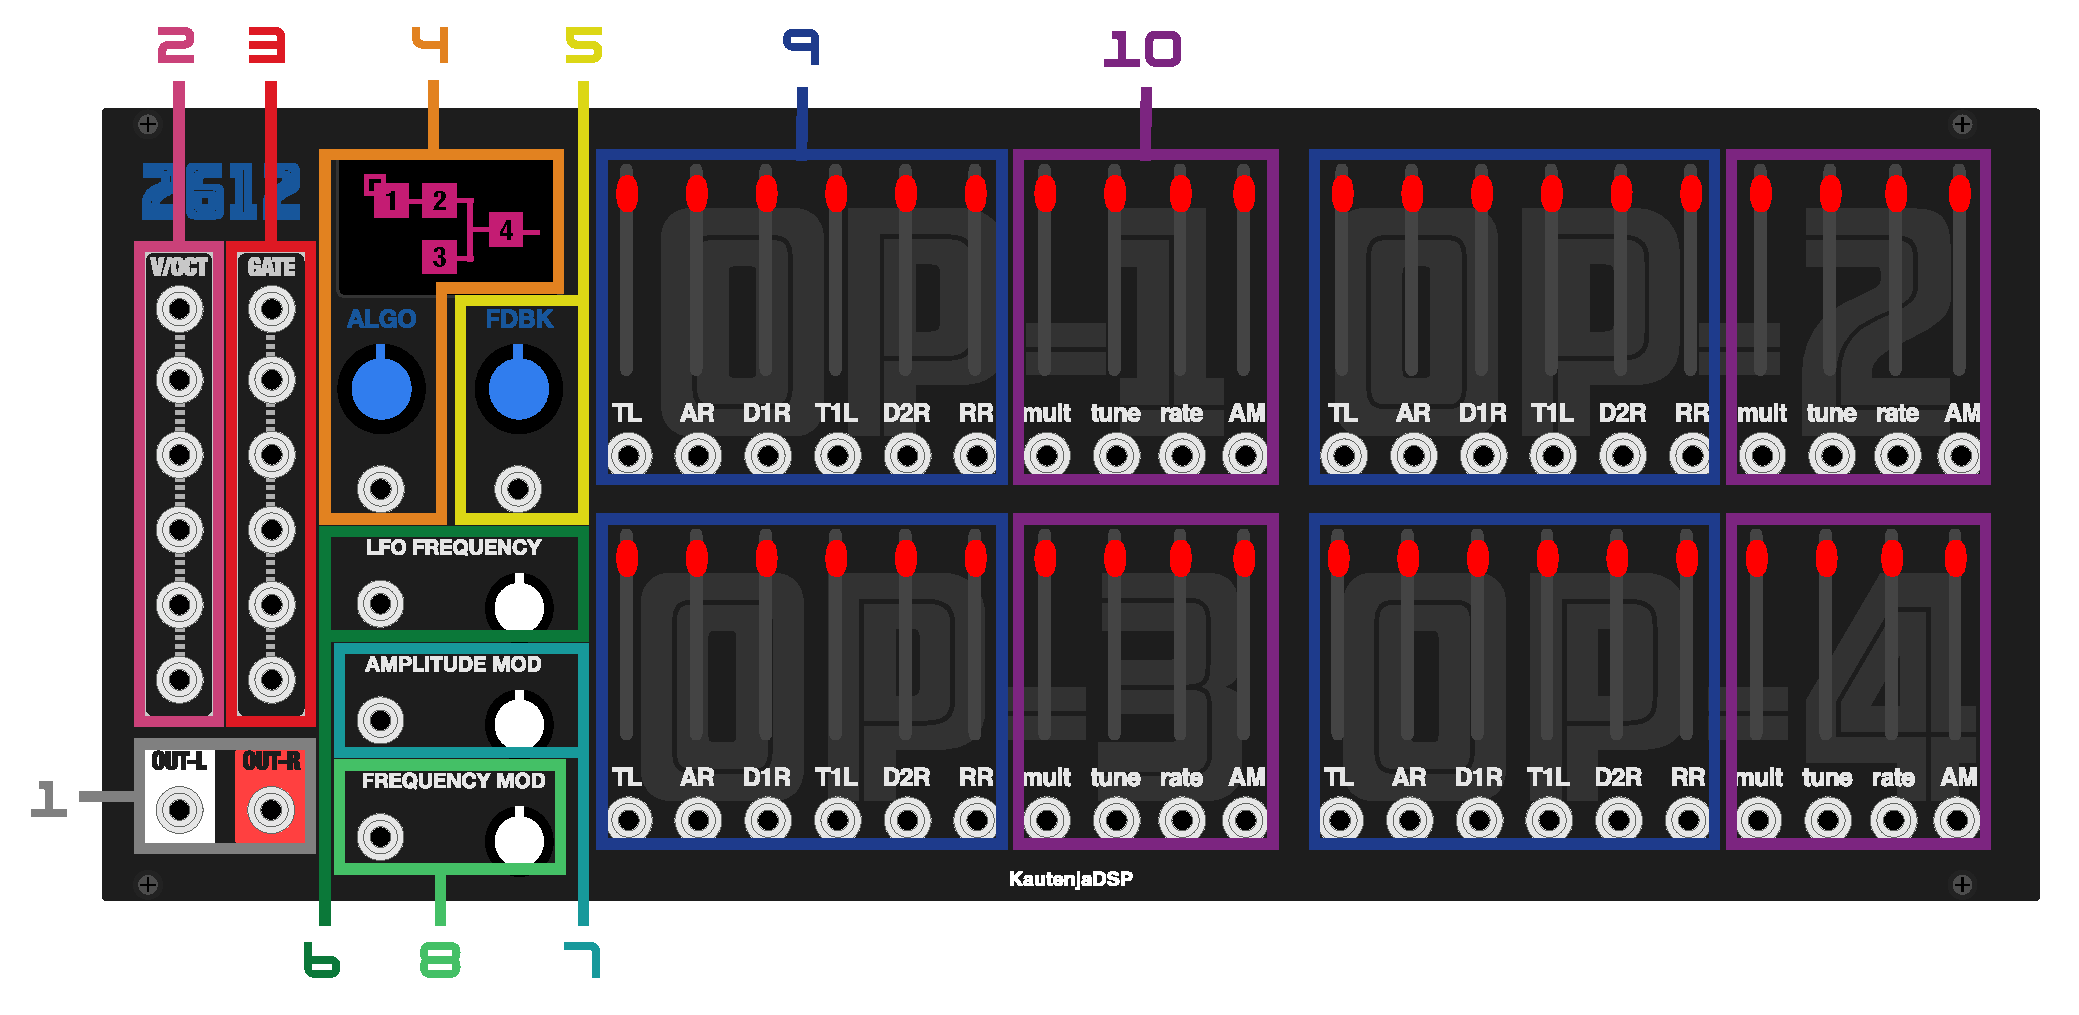
\includegraphics[width=\maxwidth{\textwidth}]{2612-Manual}
\end{figure}

\begin{figure}[!htp]
\centering
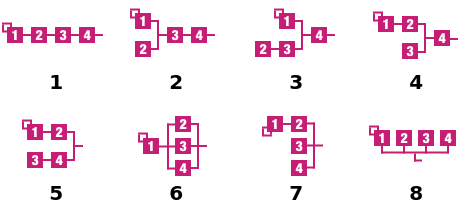
\includegraphics[width=\maxwidth{\textwidth}]{2612-Operators}
\caption{An illustration of the FM algorithms on the module.}
\label{fig:fm-algorithms}
\end{figure}

\begin{figure}[!htp]
\centering
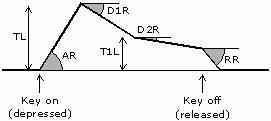
\includegraphics[width=\maxwidth{\textwidth}]{envelope}
\caption{An illustration of the stages in the envelope generator.}
\label{fig:envelope-generator}
\end{figure}

\clearpage
\begin{enumerate}
  \item Stereo master output from the module
  \item $V$/Octave inputs for each of the 6 synthesizer voices.
  \item Gate inputs for each of the 6 synthesizer voices. The gate goes high at $2V$ and triggers the envelope generators on the module. Figure~\ref{fig:envelope-generator} illustrates how the enveloper generator interprets the gate signal.
  \item Algorithm selector and display. The YM2612 offers eight distinct FM synthesis algorithm based on the four operators on the module. Figure~\ref{fig:fm-algorithms} describes the configuration of the operators for each of the algorithms.
  \item Feedback control for operator 1. The value of this parameters determines how much the output of operator 1 feeds back into itself.
  \item Frequency control for the global LFO. TODO
  \item Global amplitude modulation control. TODO
  \item Global frequency modulation control. TODO
  \item Control over the envelope generator parameters for each of the four operators on the module. Figure~\ref{fig:envelope-generator} depicts the stages in the envelope generator. \begin{enumerate}
    \item \textbf{Total Level (\texttt{TL}):} The highest amplitude of the envelope generator
    \item \textbf{Attack Rate (\texttt{AR}):} The angle of initial amplitude increase. This can be made very steep if desired. The problem with slow attack rates is that if the notes are short, the release (called \texttt{key off}) occurs before the note has reached a reasonable level.
    \item \textbf{Decay Rate 1 (\texttt{D1R}):} The angle of initial amplitude decrease from the highest point in the envelope generator.
    \item \textbf{Total Level 1 (\texttt{T1L}):} The amplitude where the second decay stage starts
    \item \textbf{Decay Rate 2 (\texttt{D2R}):} The angle of secondary amplitude decrease. This will continue indefinitely unless \texttt{key off} occurs.
    \item \textbf{Release Rate (\texttt{RR}):} The final angle of amplitude decrease, after \texttt{key off}.
  \end{enumerate}
  \item Control over the FM parameters for each of the four operators on the module. \begin{enumerate}
    \item \textbf{Multiplier:} TODO
    \item \textbf{Tuning:} TODO
    \item \textbf{Rate Scale:} the degree to which envelopes become shorter as frequencies become higher. For example, high notes on a piano fade much more quickly than low notes.
    \item \textbf{Amplitude Modulation:} Whether amplitude modulation is enabled for the given operator. The amplitude modulation is controlled by the global LFO.
  \end{enumerate}
\end{enumerate}

% -------------------
% MARK: References
% -------------------

\clearpage
\renewcommand\refname{References \& Acknowledgments}
\nocite{*}
\bibliographystyle{apalike}
\bibliography{references}

\end{document}
